\documentclass{beamer}
\usepackage[utf8]{inputenc}
\usetheme{Darmstadt}

\usepackage{times}
\usefonttheme{structurebold}

\usepackage{pgf}
\usepackage{tikz}
\usepackage{alltt}
\usepackage{url}
\usepackage[absolute,showboxes]{textpos}
\usetikzlibrary{arrows}
\usetikzlibrary{shapes}
\usetikzlibrary{automata}
\usetikzlibrary{calc}
\usepackage{amsmath,amssymb}

\title{Technical Presentation Milestone Presentation}
\author{Patrick~Lam\\Department of Electrical and Computer Engineering}
\date{December 1, 2009}

\begin{document}

\newcommand{\CcNote}[1]{% longname
	This work is licensed under the \textit{Creative Commons #1 3.0 License}.%
}
\newcommand{\CcImageBy}[1]{%
	
\includegraphics[scale=#1]{creative_commons/cc_by_30.pdf}%
}
\newcommand{\CcImageSa}[1]{%
	
\includegraphics[scale=#1]{creative_commons/cc_sa_30.pdf}%
}
\newcommand{\CcGroupBySa}[2]{% zoom, gap
	\CcImageBy{#1}\hspace*{#2}\CcImageSa{#1}%
}
\newcommand{\CcLongnameBySa}{Attribution-ShareAlike}

\begin{frame}
  \titlepage

  \vfill
  \begin{center}
    \CcGroupBySa{0.83}{0.95ex}\\
		  {\tiny\CcNote{\CcLongnameBySa}}
		  \vspace*{-2.5ex}
  \end{center}

\end{frame}

\section*{Outline}
\begin{frame}
  \tableofcontents
\end{frame}

\section[TPM]{The Technical Presentation Milestone: Mechanics}

\begin{frame}
\frametitle{Webpages}

\begin{itemize}
\item[] {\large
\url{http://patricklam.ca/tpm}
}\\
My TPM page for Software Engineering students\\[2em]

\item[] {\large 
\url{http://www.ece.uwaterloo.ca/~tppe000/}
}

TPM page by Prof. Harder for ECE students
\end{itemize}

\end{frame}

\begin{frame}
\frametitle{Why the TPM?}

\Large
Co-op employers:

\begin{center}
``UW students cannot give presentations.''
\end{center}

\end{frame}

\begin{frame}

\frametitle{When?}

\begin{center}
{\Large 2B}
\end{center}

\end{frame}

\begin{frame}

\frametitle{What's in a TPM presentation?}

Technical presentation, normally related to your 2B work term.

\begin{itemize}
\item 12-15 minutes (with slides);
\item 5 minutes question-and-answer; 
\item 2 evaluators and a peer audience.
\end{itemize}

\end{frame}

\begin{frame}

\frametitle{What should I talk about?}

\Large
Explain something you know (well).\\[2em]

Show enthusiasm!

\end{frame}

\begin{frame}

\frametitle{Purpose}

\Large
Goal: Inform or persuade.\\[2em]

Your presentation is not:
\begin{itemize}
\item a sales pitch;
\item your work report in slide form.
\end{itemize}
~\\[1em]

Level: appropriate for 2B students.

\end{frame}

\begin{frame}

\frametitle{Evaluation}

\begin{itemize}
\item 4 criteria, each marked out of 2:
\begin{itemize}
\item organization;
\item quality of overheads;
\item presentation style;
\item response to questions.
\end{itemize}
\item 2 markers; your total is the sum of marks
\item to pass, you need 12/16 with at least 1 for each criterion
\end{itemize}

\end{frame}

\begin{frame}

\frametitle{Hoops I}

Time and Place: \\
$\qquad$ MW 2:30-5:30 in EIT3145\\[2em]

Sign ups: \\
$\qquad$ on Quest for TPM 1X000.\\[2em]

Bring your .ppt or .pdf file.\\[1em]

Dress appropriately and attend all talks in your session.\\[1em]

Pick up your evaluation a week after the presentation.

\end{frame}

\begin{frame}

\frametitle{Hoops II}
\Large

Three Required Slides:
\begin{itemize}
\item Title Slide: title, name, date
\item Outline
\item Summary
\end{itemize}

\end{frame}

\begin{frame}
\frametitle{Timer}

\begin{columns}[c]
\column{.5\textwidth}
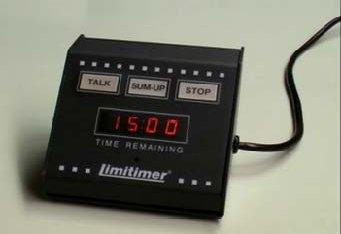
\includegraphics[width=\columnwidth]{before}\\
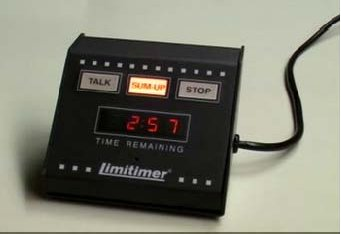
\includegraphics[width=\columnwidth]{wrapup}
\column{.5\textwidth}
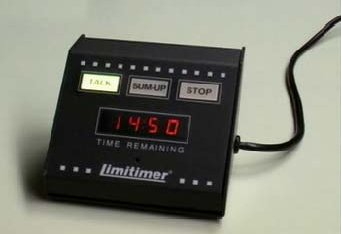
\includegraphics[width=\columnwidth]{during}\\
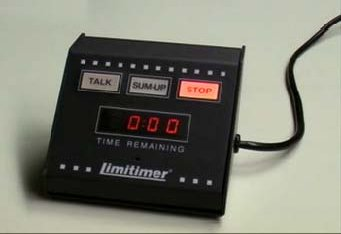
\includegraphics[width=\columnwidth]{stop}
\end{columns}

\end{frame}

\begin{frame}

\frametitle{Recovery Options}

If you fail: \\
$\quad$ Try again in 3A.\\[2em]

If you fail again:\\
$\quad$ See the Associate Director for more options.\\[2em]

You may not register for 3B until you fulfill this milestone.

\end{frame}

\begin{frame}

\frametitle{Example TPM Presentations}

\url{http://www.ece.uwaterloo.ca/~tppe000/Examples/}

\small
\begin{itemize}
\item Comparison of PostgreSQL and MySQL/InnoDB\\
$\qquad$(Baverstock)
\item How Apple's launchd Compares to a Standard System V init\\
$\qquad$(Zarnett)
\item Network Security---Passive and Active Methodologies\\
$\qquad$(Robinson)
\item Next Generation Optical Media\\
$\qquad$(Armstrong)
\end{itemize}



\end{frame}


\section{Presentation Skills}

\begin{frame}

\end{frame}

\subsection{Planning}
\subsection{Telling}
\subsection{Showing}
\subsection{Answering Questions}

\section{On Presentation Styles}

\begin{frame}
\frametitle{The Cognitive Style of PowerPoint}

\end{frame}

\begin{frame}
\frametitle{Gettysburg Address}

\end{frame}

\begin{frame}
\frametitle{Lessig Style}
\end{frame}

\section{Conclusion}

\begin{frame}
\frametitle{Summary}

Described the format of the Technical Presentation Milestone.\\[1em]

Gave tips on presentations:

\begin{itemize}
\item planning;
\item speaking;
\item organizing slides; and
\item answering questions.
\end{itemize}


\end{frame}

\end{document}


